%\documentclass[tikz, border=5pt]{standalone}
\usetikzlibrary{angles, quotes} % 用于绘制角度标记
\begin{document}
	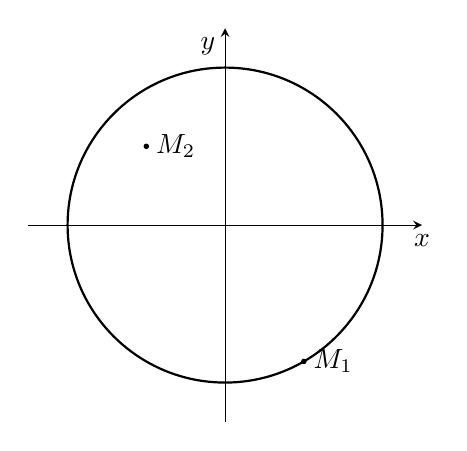
\begin{tikzpicture}[>=stealth, scale=0.5] % 缩放使图形更清晰
		
		% 绘制坐标轴
		\draw[->] (-5,0) -- (5,0) node[below] {$x$};
		\draw[->] (0,-5) -- (0,5) node[below left] {$y$};
		
		% 绘制圆
		\draw[thick] (0,0) circle (4);
		
		\fill ({4*cos(-60)}, {4*sin(-60)}) circle (2pt) node[ right] {$M_1$}; % 圆上的交点
		\fill(-2,2) circle (2pt) node[ right] {$M_2$}; 
		
	\end{tikzpicture}
\end{document}
